\subsection*{Problema 31}
\textbf{Enunciado:} Calcular la integral:
\begin{align*}
\int \dfrac{2x^2 + 3x - 1}{x^3 + 2x^2 + 4x + 2} \, dx
\end{align*}

\textbf{Solución:}
Primero, analizamos el denominador 
$P(x) = x^3 + 2x^2 + 4x + 2$. 
Buscamos raíces racionales usando los divisores del término constante ($2$), los cuales son $\pm 1, \pm 2$. Evaluando en $x = -1$:
\begin{align*}
P(-1) &= (-1)^3 + 2(-1)^2 + 4(-1) + 2 \\
&= -1 + 2 - 4 + 2 = -1 \neq 0
\end{align*}
Probamos agrupando términos o usando división sintética. Notemos que si factorizamos por división:
\begin{align*}
x^3 + 2x^2 + 4x + 2 = (x+1)(x^2 + x + 2)
\end{align*}
El trinomio $x^2 + x + 2$ tiene un discriminante negativo ($\Delta = 1^2 - 4(1)(2) = -7$), por lo que es irreducible en los reales.

Planteamos la descomposición en fracciones parciales de la siguiente manera:
\begin{align*}
\dfrac{2x^2 + 3x - 1}{(x+1)(x^2 + x + 2)} &= \dfrac{A}{x+1} \\
&+ \dfrac{Bx + C}{x^2 + x + 2}
\end{align*}

Multiplicando toda la expresión por el denominador común, obtenemos:
\begin{align*}
2x^2 + 3x - 1 &= A(x^2 + x + 2) \\
&+ (Bx + C)(x+1)
\end{align*}

Evaluamos en $x = -1$ para hallar $A$:
\begin{align*}
2(-1)^2 + 3(-1) - 1 &= A((-1)^2 + (-1) + 2) \\
2 - 3 - 1 &= A(1 - 1 + 2) \\
-2 &= 2A \implies A = -1
\end{align*}

Expandimos y agrupamos términos para $B$ y $C$:
\begin{align*}
2x^2 + 3x - 1 &= Ax^2 + Ax + 2A \\
&+ Bx^2 + Bx + Cx + C \\
&= (A+B)x^2 + (A+B+C)x \\
&+ (2A+C)
\end{align*}

Igualando coeficientes:
\begin{align*}
A + B &= 2 \implies -1 + B = 2 \implies B = 3 \\
2A + C &= -1 \implies 2(-1) + C = -1 \implies C = 1
\end{align*}

Sustituimos los valores hallados en la integral original:
\begin{align*}
\int &\left( \dfrac{-1}{x+1} + \dfrac{3x + 1}{x^2 + x + 2} \right) dx
\end{align*}

Integramos el primer término directamente:
\begin{align*}
\int \dfrac{-1}{x+1} \, dx = -\ln|x+1|
\end{align*}

Para el segundo término, derivamos el denominador: $\frac{d}{dx}(x^2+x+2) = 2x+1$. Ajustamos el numerador:
\begin{align*}
\dfrac{3x+1}{x^2+x+2} &= \dfrac{\frac{3}{2}(2x+1) - \frac{3}{2} + 1}{x^2+x+2} \\
&= \dfrac{\frac{3}{2}(2x+1) - \frac{1}{2}}{x^2+x+2}
\end{align*}

Separamos en dos integrales:
\begin{align*}
\int \dfrac{\frac{3}{2}(2x+1)}{x^2+x+2} \, dx &= \dfrac{3}{2}\ln|x^2+x+2| \\
\int \dfrac{-\frac{1}{2}}{(x+\frac{1}{2})^2 + \frac{7}{4}} \, dx &= -\dfrac{1}{2} \cdot \dfrac{2}{\sqrt{7}}\arctan\left(\frac{x+\frac{1}{2}}{\frac{\sqrt{7}}{2}}\right)
\end{align*}

Uniendo todos los resultados y agregando la constante de integración $C$:
\begin{align*}
F(x) &= -\ln|x+1| + \dfrac{3}{2}\ln(x^2+x+2) \\
&- \dfrac{1}{\sqrt{7}}\arctan\left(\frac{2x+1}{\sqrt{7}}\right) + C
\end{align*}

\begin{figure}[H]
	\centering
	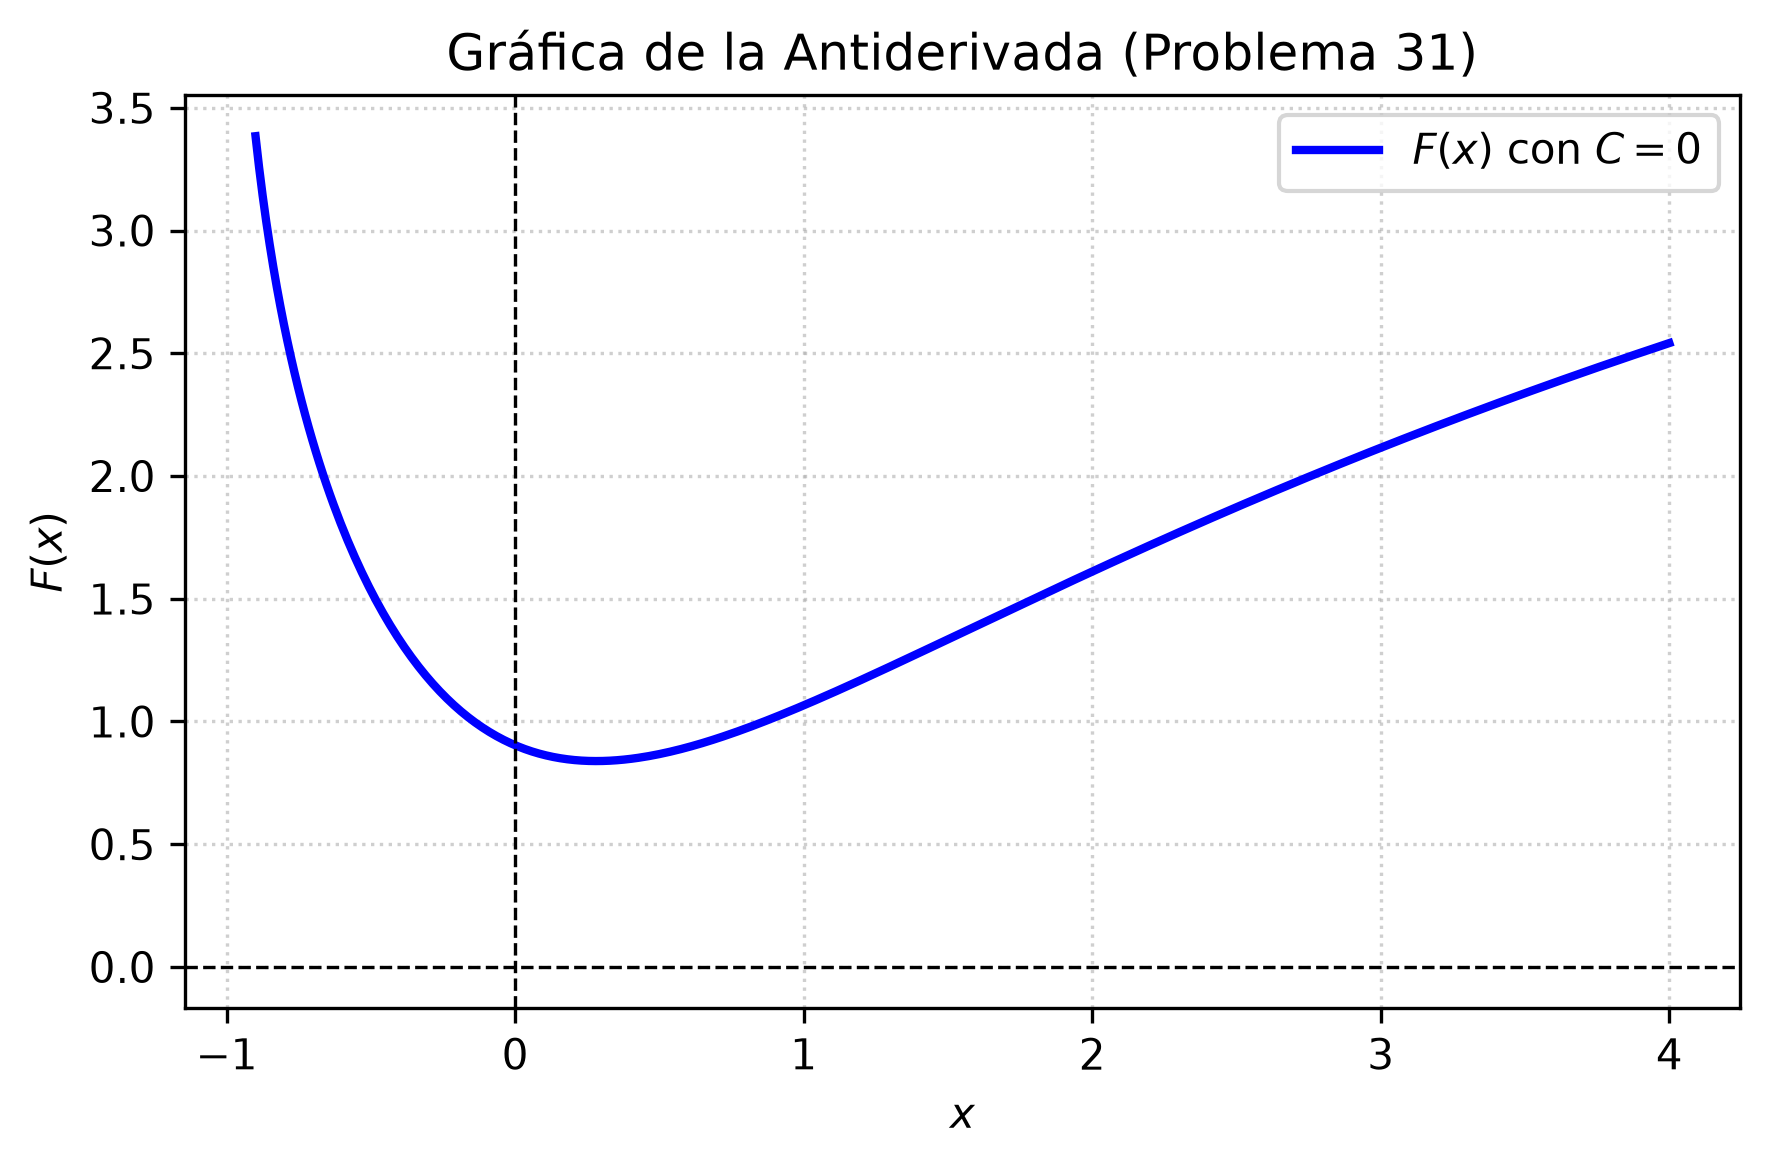
\includegraphics[width=\columnwidth]{semana_03/graficas/SEM03_P31_grafica.png}
	\caption{Representación gráfica de $f(x)$ y su antiderivada $F(x)$ evaluada para la constante de integración $C = 0$ (Problema 31).}
	\label{fig:problema31}
\end{figure}
